\documentclass[12pt]{article}
\usepackage[breaklinks=true]{hyperref}
\usepackage[margin=1in]{geometry}
\usepackage{graphicx}
\usepackage{color}

\definecolor{pblue}{rgb}{0.13,0.13,1}
\definecolor{pgreen}{rgb}{0,0.5,0}
\definecolor{pred}{rgb}{0.9,0,0}
\definecolor{pgrey}{rgb}{0.46,0.45,0.48}

\usepackage{listings}
\lstset{language=Java,
  showspaces=false,
  showtabs=false,
  tabsize=2,
  breaklines=true,
  showstringspaces=false,
  breakatwhitespace=true,
  commentstyle=\color{pgreen},
  keywordstyle=\color{pblue},
  stringstyle=\color{pred},
  basicstyle=\ttfamily,
  frame=single,
  moredelim=[il][\textcolor{pgrey}]{$$},
  moredelim=[is][\textcolor{pgrey}]{\%\%}{\%\%}
}

\title{Java Collections}
\author{
	Melvyn Ian Drag
}
\date{\today}


\begin{document}
\maketitle

\begin{abstract}
$java.util$ provides many containers. These containers are widely used in Java programming and are implementations of the great data structures you hear about in data structures \& algorithms classes. In today's lecture we'll have a look at a few of them and consider when we would want to use them.
\end{abstract}

\section{Exam - Last few minutes of class.}
Ask students to document code
\section{Sets}
We are going to learn about sets today.

The purpose of a set is to store exactly one copy of each item. In this regard, sets are a bit different from arrays. An array 

\textit{Illustrate the concept on the board}

To describe a set is somewhat simple ( unless you think deeply about it in terms of mathematics! ). We will just say a set is like a List, except a list can contain multiple copies ofthe same value - a set cannot. Sometimes you will want this in your code. I can't tell you when or why - you'll need to write alot of code and then some day, if you haven't had the epiphany yet, you'll have it. Sets are useful, and it is a data structure that comes up naturally in many situations when you are writing code. 

I remember when I learned about a dictionary in python - I thought it was the stupidest thing ever! Why would anyone want a to index their arrays by a string, what is wrong with a number?!?!?! A few weeks later I was working on a project and realized it would be super convenient if I could create a relationship between strings and the values they represented . . . and thus my love of the dictionary was born and I pledged to never doubt the importance of an algorithm or datastructure when someone was passionately teaching it to me.

You all might feel this way about this class or the other one I'm teaching. Like ni here, why am I making you manipulate bits, understand image formats, or study the difference between ASCII, UTF8 and UTF16. You can trust that these are important things to know and that if you don't believe me, it's because you haven't written enough programs yet! The same in my other class, the Linux class. We are setting up websites, databases, studying a handful of simple programming languages! These things are really small, simple things I'm showing, and with time, as you do bigger projects, you'll see what we're learning is just the tip of the iceberg!

We are only together for a few weeks in this class, but you will spend the rest of your life as a programmer! You should learn these concepts now and then get ready to continue learning way harder concepts for the rest of your career! Some jobs like accounting and construction are kind of mentally simple - the same thing, over and over again. The same tools. The jobs are incredibly challenging, but don't require too much creativity. Programming on the other hand requires you to have some basic level of love and understanding of math, and then learn a million languages and circuit boards, processors, etc, and deliver on ridiculously short timelines. 

Back to the lecture - there are a bunch of types of sets that one can learn about in a data structures class. Java implements many many types of sets. Today we will have a peek at three of them in no great detail, but just so that you know they are there and more or less what they do.

\begin{enumerate}
\item HashSet
\item TreeSet
\item LinkedHashSet
\end{enumerate}

Set is the interface that all of these implementations implement. Now you understand it's most essential feature - a set is like a list, but it only stores unique elements, no duplicates! 

\subsection{Interview Warning}
When you go for your big interview at Amazon ( and I only mention amazon because they are hiring Java and Linux experts both in Newark and New York City! ), you may have a problem that requires you to maintain some unique set of elements. For example, here is a basic interview question:

{\Large\textit{Given an array, how can you remove all duplicates?}}

to which you might rush and think ``USE A SET!!! DUH!!" but there is more to the problem than this. ArrayLists and LinkedLists are naturally ordered! You know who is first and who is last - but do you know this information when you use a set? I'll show you a bit about sets now and talk a tiny tiny tiny bit about theory, but ultimately you need to take a few semesters of algorithms to understand the answer to this problem!

\section{War Story}
If you look in Steve Skiena's "The Algorithm Design Manual" he includes "war stories" throughout the book about his experiences in industry. I'm begging the department here to let me teach an algorithms class because I haven't read that book in a few years and I'd like an excuse to review it. Anyway, heres an industry story of mine:

Today we are talking about HashSets and TreeSets. These are intimately related to two other datastructures called HashMaps and TreeMaps. In fact, HashSets are built on HashMaps and TreeSets are built on TreeMaps. You can see the references below.

\subsection{References}
\begin{enumerate}
\item \url{https://www.baeldung.com/java-tree-set}
\item \url{https://www.baeldung.com/java-hashset-vs-treeset}
\item \url{https://www.baeldung.com/java-hashset}
\end{enumerate}

Anyway, we were working on a Kidney Dialysis Machine at DEKA in Manchester NH.
\url{https://www.fiercebiotech.com/medtech/cvs-kicks-off-first-trial-its-home-dialysis-device}. The machine is now being tested by CVS on patients. I wrote some of the code in that machine! It's C++ code that communicates between a circuit board in the device and a database. I'm really proud of it, and you have to keep studying computer science so you can get your code inside cool machines, or make cool websites, or whatever. 

Anyway, I needed a map. I was a bit lazy and didnt read the documentation, so I chose a "map" fro the standard library. \url{http://www.cplusplus.com/reference/map/map/} There is whdre it's described. And we wrote the code and tested it and whatever, no big deal everything worked. The thing about these machines is that they are very complicated and the timing of events in the machine has to be very precise. The machine is connected to a patient's veins and takes their blood out. Inside the machine it has to pump the blood through a series of filters and measuring devices to make sure the blood has been piurified of toxins. Then it pumps the blood back into the patients veins and where it goes to the patient's heart and is recirculated through his or her body. The timing of all these pumps needs t obe very very precise or else the machine could fail and kill a patient ( in the worst case scenario ).

The database code I wrote stored some data in a map and in testing everything was going fine. One day, disaster struck and the operation that was supposed to take 100milliseconds started taked 300milliseconds.

I poured over my code with a buddy we ran weeks and weeks of tests. Then, ifnally, it hit us. We shouldhave been using a different datastructure called an unordered\_map. You can read abot it here: \url{http://www.cplusplus.com/reference/unordered_map/unordered_map/}. The map I had been using was based on trees and comparators. You can see it in the documentation - \textit{show the constructor}, but I had meant to use a map that was based on a hash - this is the unordered\_map \textit{Show the documentation.}

My buddy Brian figured out the error, we changed it, and then everything worked out. And now that code is running on a machine that is improving the qualitiy of life of the poor people with late stage kidney failure. 

The message here is choose the right datastructure. If we hadn't found that bug, the project would have been very delayed as I would have had to rewrite the whole logic of a program that was performing a critical function. Pay attention in school, get familiar with different datastructures, and choose the right one when you start working. We are learning Java here tonight, and two things we will learn are HashSets and TreeSets, which are similar to the map and unordered map I just discussed from C++. Then Ill show you an even cooler datastructure called a LinkedHashMap. So let's begin.


\section{What is a HashSet?}

\subsection{What is a hash function}
Generally a hash function is just a function, but you expect the hash function to have some particular properties. 

You see hash functions all over the place in computer science. Often times, programmers like us use hash functions to generate a small string from a large file. We use things like md5sums, which are hash funtions. Commit this to memory! \textbf{md5sum}! This particular hash is used by programmers all the time, day after day after day. An example of a use case is if I want to give you a pdf to read. I will also give you the md5sum. Before you open the pdf, you run the file through a program that can compute the md5sum. If the md5sum is the same, that means the input to the function was the same and you can trust the file. If te md5sum is different, that means that the input to the md5sum function was different and you shouldnt trust the file.

{\LARGE\textit{show alchemistowl \url{https://www.alchemistowl.org/pocorgtfo/}and \url{http://releases.ubuntu.com/trusty/} the link for downloading the Ubuntu linux operating system. Whenever you download a file, you should also get the hash of the file and verify the hash is correct before you install or use the thing from the internet. There are viruses on the internet created by bad people! Programmers like us always provide a way to verify that we aren't downloading viruses.}}

Now, in this class we are using these functions that generate an output for a given input to do a different task. We need the hash function to output a number. We use that number as a n array index

There is alot of algorithmic research that goes into designing great hash functions. I'll tell you about it via an example.  Look at the following two examples to see how a hash set works and to see if the objects are 

\subsection{An example}
This shows how you add elements to a hashset. Note that the add() method for sets return a boolean indicating whether or not the element was already in the collection.

\url{https://docs.oracle.com/javase/7/docs/api/java/util/Set.html}

\lstinputlisting{Code/HashSetTest.java}

\subsection{Another Example}
Hash sets do not maintain the order of the elements that were inserted. Revisit the previous example, but insert the elements in a different order. You will note that the output of the program is exactly the same.
\lstinputlisting{Code/HashSetOrdering.java}

\subsection{A Question For You}
The add method is from the Collections interface. So we would expect List to return a bool from the add Method.

\url{https://docs.oracle.com/javase/7/docs/api/java/util/List.html#add(E)}

According to the docs above, what bool value is returned?

\section{What is a TreeSet?}
A tree set is another implementation of Set like a HashSet, but a TreeSet is stored in sorted order. As I said before, Java has many set implementations. I have no idea when or where in your life and career you'll want one or the other. I'm just showing you three of them now that I thought were interesting. They all do the same thign - they all store data without duplicates, but how they do it is different and the Set you use may impact the performance of your code.

Here is a good description I found of TreeSet on the internet.

\begin{figure}[h]
  \centering
    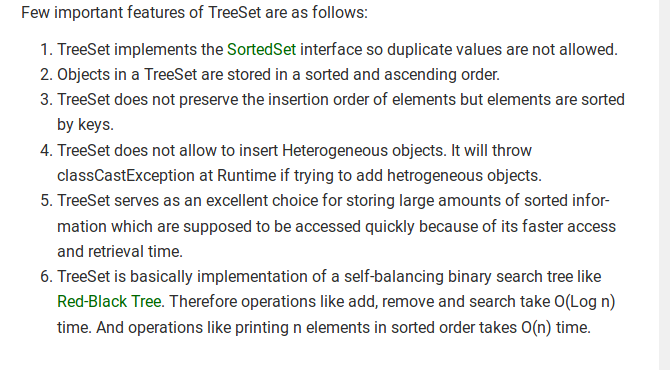
\includegraphics[width=0.8\textwidth]{Images/treeSet.png}
  \caption{\url{https://www.geeksforgeeks.org/treeset-in-java-with-examples/}}
\end{figure}

Take away: the HashSet should be fast, but does not retain insertion order. It also doesn't sort the elements. The tree set does not remember insertion order, it is probably a bit slower than the HashSet for some operations, but does keep it's contents sorted.

\subsection{What is a tree}
An array is an easy thing to explain as a datastructure. An ArrayList is the same thing , it can just grow. A LinkedList is also easy to understand. Elements aren't adjacent in memory as with an Array, but they have pointers to each other to know who comes first and second and third and so forth. These two datastructures correspond directly to hardware and you can think of them in memory. 

A tree is a bit more abstract. We can describe a tree on paper, but then to implement a tree - we have many choices when we think about how we'll do it in memory. In general, we are intersted in Binary Searched Trees ( BSTs ) in computer science. \textit{Draw a BST on the board. Make it unbalanced.}

But even more interesting than BSTs to us as computer scientists are Balanced Binary Search Trees, whic are like the one I've just drawn, but the depth of all hte branches is approximately equal. \textit{Correct the BST on the board to make it balanced.}

{\LARGE\textit{Do you know any implementatoins of Balanced Binary Search Trees? Ask a few kids who have taken algorithms and data strucutres already}}

So according to the very little research I did, the TreeSet in java uses a BBST called a ``Red-Black Tree". Go through an example of how 


\subsection{An example}
\lstinputlisting{Code/TreeSetTest.java}


\subsection{Another Example}
Verify that the TreeSet does indeed maintain the Set in sorted order. Add a bunch of strings to the set and make sure that the strings always come out in sorted order.
Redo this experiment with the HashSet to verify that the HashSet does not return sorted elements.


\section{Exercise  \#1 - Difference Between a HashSet and a TreeSet}
In the Ordering examples I showed you, the HashSet and TreeSet return the values in the same order. Im telling you though - HashSets are not sorted. Can you give an input to the Hash and TreeSets so that when I iterate over them, the order of elements is different?

\section{Exercise \#2 - Reversing a Tree Set}
According to my research, TreeSet has a constructor that allows you to supply a comparator. As we've seen so far, our tree set is sorted such that the strings that are lower in the alphabet come first. Like "Hello" comes before "World". Let's take 10 minutes and see who can research the fastest in this class. What is a Comparator? How do you create on? TreeSet has a method called "descendingSet()" - if that returns a Set then we are good. If you can figure this out quickly, can you implement a custom comparator that always puts anything with an "A" first and then sorts the rest in some other order?

\textbf{Create a Tree Set with the Strings inside stored in reverse order}

\begin{lstlisting}
Set<T> t = new TreeSet<T>(Comparator c);
\end{lstlisting}

Might be helpful, I don't know:
\url{https://stackoverflow.com/questions/32995559/reverse-a-comparator-in-java-8}

\section{What is a LinkedHashSet?}
A LinkedHashSet is like a HashSet, but in addition to computing where data is stored and if data is present with a Hash function, it also maintains a linked list of allthe elements in the container, so it can also tell you the order of insertion in addition to some additional things about your data. I haven't tested this collection extensively, but I would expect it to be slower than a HashSet for some operations because it has to compute a hash, store data but then ALSO update a linked list. Then again, some operations will be faster thanks to the linked list. We would expect the LinkedHashSet to consume more memory than a HashSet.

\subsection{Test it out}

\subsection{Check out ordering}

\subsection{Activity}
The LinkedHashSet should consume more memory than a HashSet. Just for fun, let's check out our computer and see if that is true.

Write two programs. One stores 10000 values in a HashMap, the other in a LinkedHashMap. use htop or task manager to see which one takes more RAM.


\section{Grades}
Grades are not an evaluation of your soul or worth as a human being. Grades are an evaluation of your knowledge of Java.  Show the Francis Su presentation.

\section{If Extra Time}
What is a leap second? When will the next one be? Is there a scheduled one coming up? We might have a party and watch the clocks and try and generate a programatic error at the leap second!

\section{If extra time: start working on homework}

\end{document}
